\chapter{Kiến thức nền tảng}
\label{chap-background}
\begin{ChapAbstract}
Trong chương này, nhóm sinh viên trình bày các kiến thức nền tảng liên quan tới mạng Neural Networks, bao gồm các kiến trúc căn bản, cấu trúc một số Deep Neural Networks phổ biến và các cấu trúc mạng Recurrent Neural Networks.
\end{ChapAbstract}

\section{Neural Networks}
\subsection{Giới thiệu về Neural Network và Deep Learning}
Hiện nay, Deep learning là kĩ thuật hay được nhắc tới nhất khi giải quyết các bài toán thị giác máy tính trên ảnh, video và ngôn ngữ do Deep Learning mang lại những kết quả vượt trội so với những phương pháp truyền thống. Thành phần nền tảng cơ bản nhất mà Deep Learning dựa vào để phát triển là Neural Network. Neural Network, một khái niệm nền tảng trong lĩnh vực máy học nói riêng và trí tuệ nhân tạo nói chung, là một nỗ lực thiết kế một thuật toán phân lớp lấy cảm hứng từ cấu tạo sinh học của neural trong não động vật. Cụ thể hơn,trong Neural Network, các neural liên kết với nhau tạo thành một mạng, và mạng này học bằng cách điều chỉnh trọng số của các kết nối giữa các neuron với nhau. Chính vì điều này, Neural Network còn được gọi tên là Mạng Neuron nhân tạo (Artificial Neural Networks - ANNs). Thực tế, Neural Network đầu tiên được hai nhà nghiên cứu McCulloch và Pitts đề xuất năm 1943, là một ví dụ đơn giản nhất của Neural Network. Mạng này là một loại phân lớp tuyến tính, có khả năng phân biệt hai lớp dữ liệu là dương tính hay âm tính. Năm 1950s, Rosenblatt đề xuất ra một perceptron, trở thành mô hình đầu tiên có khả năng học trọng số từ những ví dụ trong tập huấn luyện. Cũng cùng khoảng thời gian này, phần tử adaptive linear element (ADALINE) trở thành mô hình đầu tiên có thể dự đoán một số thực từ việc học từ dữ liệu huấn luyện.

Tuy nhiên, những mô hình tuyến tính như perceptron và ADALINE là những mô hình phân lớp tuyến tính. Tức là những mô hình này có khả năng phân lớp, dự đoán tốt với những dữ liệu có thể phân tách bằng một siêu phẳng tuyến tính. Còn lại, đối với những dữ liệu không thể phân tách được bằng một mô hình siêu phẳng tuyến tính, thì những mô hình này còn thể hiện sự hạn chế. Một ví dụ điển hình nhất về sự hạn chế này là hàm $XOR$, khi $ XOR(0,1) = XOR(1,0) = 1 $, $XOR(1,1) = XOR(0,0) = 0$. Ta không thể chỉ ra một đường thẳng (siêu phẳng tuyến tính trong không gian hai chiều) để phân lớp kết quả output của hàm này. Chính vì sự giới hạn này, Neuron Network trong một thời gian dài không được dành được sự chú ý. 

Cho tới tới năm 2006, Geoffrey Hinton trình bày một neural network được gọi là Deep Belief Network có thể được huấn luyện bằng một chiến thuật gọi là greedy layer-wise pre-training. Khái niệm Deep learning bắt đầu từ công trình này, do công trình này chứng tỏ những mạng neuron sâu nối tiếp nhau có thể được huấn luyện, và lần lượt những công trình tiếp sau đó chứng tỏ sự quan trọng của độ sâu mạng.Tính tới thời điểm này, dựa vào sự phát triển về cấu trúc và các mô hình của Deep Learning cùng với sự phát triển của các tập dữ liệu đã làm cho Deep Learning trở nên vượt trội so với những phương pháp truyền thống của Machine Learning trong nhiều công việc khác nhau.

\subsection{Kiến trúc, các thành phần cơ bản của mạng Neuron }
Kiến trúc cơ bản nhất của một mô hình Deep Learning là mạng truyền thẳng hay còn gọi là mạng perceptron nhiều lớp (MLP). Mạng perceptron nhiều lớp thực chất là một hàm toán học ánh xạ tập input thành tập output. Hàm này thực chất là một hàm hợp của nhiều hàm đơn giản khác nhau. Mỗi hàm khác nhau cho ta cách biểu diễn dữ liệu input khác nhau. Mục đích của mạng perceptron nhiều lớp là tìm ra những hàm đơn giản phù hợp và hợp để tạo ra hàm phức tạp hơn ánh xạ từ dữ liệu từ đầu vào tới đầu ra mong muốn. Mô hình perceptron nhiều lớp truyền thẳng, nghĩa là mô hình này gồm nhiều lớp các neural, mỗi neural từ lớp $l_{i}$ chỉ truyền thông tin một chiều tới lớp $l_{i+1}$, sao cho những liên kết này không tạo thành một chu trình. Dù mạng perceptron nhiều lớp có thể có nhiều lớp, nhưng ta có thể đặt tên cho ba phần chính của mạng này là: input layer, hidden layers, và output layer như minh họa ở hình \ref{fig:mlp} .

\begin{figure}[tb]
\centering
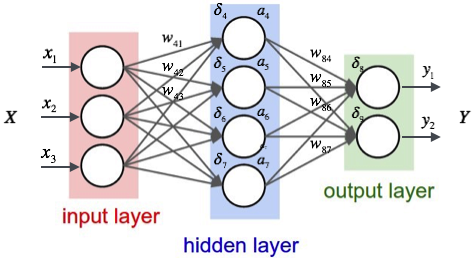
\includegraphics[]{resources/chapter2_mlp.png}
\caption{Ví dụ một mạng MLP gồm 3 thành phần input layer, 1 hidden layer và output layer}
\label{fig:mlp}
\end{figure}

Như vậy, một mạng neural truyền thẳng có thể xem như một hàm ánh xạ từ tập input sang tập output: $$y = f_{\Theta}(x) $$

Mỗi neural $a_{i}^{(l)}$, với $l$ là số thứ tự của layer của neural, $i$ là số thứ tự của neural trong layer hiện tại, nhận tín hiệu từ tất cả các neural $a_{k}^{(l-1)}$ của layer liền trước đó. Ta có thể xem đây là một hàm như sau: $$ a_{i}^{(l)} = g(\Theta^{l}_{i,0} a_{0}^{l-1} +  \Theta^{l}_{i,1}a_{1}^{l-1} + ... + \Theta^{l}_{i,s_{k}}a_{s_{k}}^{l-1})  $$
Với $\Theta^{l}_{i,j}$ là trọng số của kết nối từ neural thứ j ở layer $l-1$ tới layer thứ i ở layer $l$. $s_{i}$ là số lượng neural ở layer $l_{i}$. $g(x)$ là hàm một hàm kích hoạt, thông thường là hàm sigmoid hay hàm ReLU.

Dưới dạng vector: $$  a_{i}^{l} =  g( \Theta^{l-1}a^{l-1} ) $$ 

Sự có mặt của hàm kích hoạt $g(x)$, thường là một hàm phi tuyến trong những công thức trên là để cho mạng neural có thể học được những đặc trưng phi tuyến. Như đã đề cập từ trước, các mô hình tuyến tính không thể mô hình được đặc trưng phi tuyến (ví dụ hình \ref{fig:linear_nonlinear_data}. Giả sử hàm kích hoạt này là một hàm tuyến tính, chẳng hạn hàm đồng nhất, ta có thể viết lại $ a^{l+2} = \Theta^{l+1}(a^{l+1}) =\Theta^{l+1}(\Theta^{l}a^{l}) = Wa^{l}$ với $W = \Theta^{l+1}\Theta^{l}$. Như vậy giá trị $a^{l+2}$ là một tổ hợp tuyến tính của $a^{l}$, và sự có mặt của layer $l_{l+1}$ là vô nghĩa.


\begin{figure}[htp]
\centering
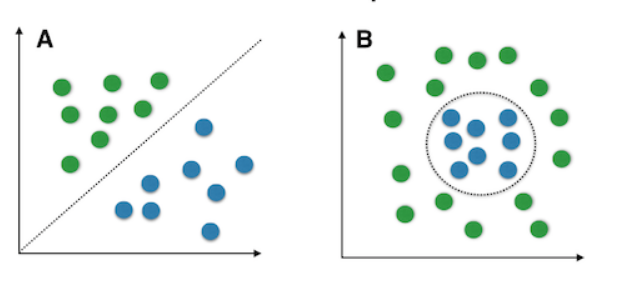
\includegraphics[width=10cm]{resources/chapter2_linear_nonlinear_data.png}
\caption[Phân lớp tuyến tính và phân lớp phi tuyến]{Phân lớp tuyến tính và phân lớp phi tuyến. \footnotesize{Nguồn: \url{https://stackoverflow.com/questions/44606126/linear-svm-vs-nonlinear-svm-high-dimensional-data}}}
\label{fig:linear_nonlinear_data}
\end{figure}


% https://stackoverflow.com/questions/44606126/linear-svm-vs-nonlinear-svm-high-dimensional-data %

Tóm lại, kiến trúc cơ bản của một mạng MLP có những điều sau đây cần lưu ý:
\begin{itemize}
\item \textbf{Giá trị của mỗi neural}: Là giá trị của hàm kích hoạt của tổ hợp tuyến tính giữa của giá trị các neural ở lớp liền trước.
\item \textbf{Hàm kích hoạt}: Là một hàm thỏa các tính chất phi tuyến, đơn điệu, khả vi. Hàm kích hoạt cần có điều kiện khả vi để có thể làm cho mạng neural học được bằng thuật toán gradient descent. Tuy nhiên, có một số hàm như $ReLU$ (Rectifier Linear Unit) không hoàn toàn khả vi tại mọi điểm. $ReLU$ không liên tục tại 0, và có một vài vấn đề với các thuật toán tối ưu dựa trên phương pháp gradient descent. Tuy nhiên, $ReLU$ vẫn có thể được sử dụng bằng cách đặt giá trị đạo hàm tại 0 bằng 0. Một số hàm kích hoạt có thể kể tới như $sigmoid$, $tanH$, $softmax$, $ReLU$, $ Leaky ReLU$.... Hiện tại, hàm ReLu (hình \ref{fig:relu} thường hay được sử dụng trong các mô hình Deep Neural Network).

\begin{figure}[htp]
\centering
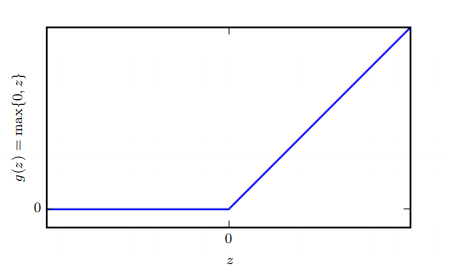
\includegraphics[]{resources/chapter2_relu.png}
\caption[Ví dụ hàm kích hoạt phi tuyến $ReLU$]{Ví dụ hàm kích hoạt phi tuyến $ReLU$. \footnotesize{Nguồn: Deep Learning Book \cite{Goodfellow-et-al-2016}}}
\label{fig:relu}
\end{figure}
% Deep Learning Book %

\end{itemize}




\begin{ChapAbstract}
Trong chương này, nhóm sinh viên đã trình bày các kiến thức nền tảng liên quan tới mạng Neural Networks, bao gồm các kiến trúc căn bản, cấu trúc một số Deep Neural Networks phổ biến và các cấu trúc mạng Recurrent Neural Networks. Các kiến thức này đóng vai trò quan trọng, làm nền tảng lý thuyết để nhóm sinh viên dựa theo và áp dụng trong chương 4 và chương 5.
\end{ChapAbstract}
